% https://tex.stackexchange.com/a/729888/322482

\documentclass[border=8pt]{standalone}
\usepackage{tikz}
\usetikzlibrary{positioning}
\makeatletter
\tikzset{
    angle/.code 2 args=\pgfmathsincos{#1}%
    \tikz@lib@place@handle@{#2}{180+#1}{\pgfmathresultx}{\pgfmathresulty}{#1}{1}
}
\makeatother
\usetikzlibrary{chains}
\tikzset{60 below left/.style={angle={240}{#1}}}
\begin{document}
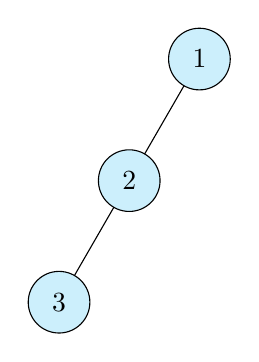
\begin{tikzpicture}[every node/.style={draw, circle, inner sep=5pt, outer sep=0pt, fill=cyan!20}]
\node (O) {$1$};
\node (A) [angle={240}{of O}] {$2$} edge (O);
\node (B) [angle={240}{of A}] {$3$} edge (A);
\end{tikzpicture}

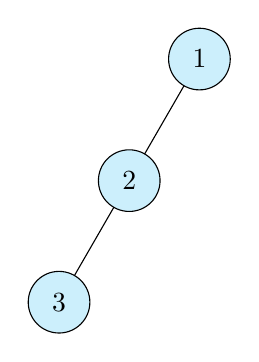
\begin{tikzpicture}[
  every node/.style={draw, circle, inner sep=5pt, outer sep=0pt, fill=cyan!20},
  start chain=going 60 below left,
  every on chain/.style={join}]
\foreach \v in {1, 2, 3}
  \node[on chain] {\v};
\end{tikzpicture}

\tikz[node distance=1.5cm and 3cm, nodes={draw, circle}, on grid]
  \draw ellipse [x radius=3cm, y radius=1.5cm] node (O) {O}
    node foreach \ang in {0, 30, ..., 359}[angle={\ang}{of O}]{\ang};
\end{document}